\documentclass[%
		%draft,
    %submission,
    %compressed,
    final,
    %
    %technote,
    %internal,
    %submitted,
    %inpress,
    reprint,
    %
    %titlepage,
    notitlepage,
    %anonymous,
    narroweqnarray,
    inline,
    twoside,
    invited
    ]{ieee}

\usepackage[utf8]{inputenc}
\usepackage[spanish]{babel}
\usepackage{graphicx}
\usepackage{verbatim}
\usepackage{moreverb}
\usepackage{amsmath}
\usepackage{amsfonts}
\usepackage{amssymb}
\usepackage{fancybox}
\usepackage{float}
\usepackage{fancyvrb}
\usepackage{subfigure}

\newcommand{\latexiie}{\LaTeX2{\Large$_\varepsilon$}}

%\usepackage{ieeetsp}    % if you want the "trans. sig. pro." style
%\usepackage{ieeetc}    % if you want the "trans. comp." style
%\usepackage{ieeeimtc}    % if you want the IMTC conference style

% Use the `endfloat' package to move figures and tables to the end
% of the paper. Useful for `submission' mode.
%\usepackage {endfloat}

% Use the `times' package to use Helvetica and Times-Roman fonts
% instead of the standard Computer Modern fonts. Useful for the 
% IEEE Computer Society transactions.
%\usepackage{times}
% (Note: If you have the commercial package `mathtime,' (from 
% y&y (http://www.yandy.com), it is much better, but the `times' 
% package works too). So, if you have it...
%\usepackage {mathtime}

% for any plug-in code... insert it here. For example, the CDC style...
%\usepackage{ieeecdc}

\begin{document}

%----------------------------------------------------------------------
% Title Information, Abstract and Keywords
%----------------------------------------------------------------------
\title[Redes de Hopfield]{%
       Redes de Hopfield}

% format author this way for journal articles.
% MAKE SURE THERE ARE NO SPACES BEFORE A \member OR \authorinfo
% COMMAND (this also means `don't break the line before these
% commands).
\author[Castiglione, Karpovsky, Sturla]{Gonzalo V. Castiglione, Alan E. Karpovsky, Martín Sturla\\\textit{Estudiantes 
       Instituto Tecnológico de Buenos Aires (ITBA)}\\
\textbf{12 de Mayo de 2012}
}


\journal{Cátedra\ \ Sist.\ de\ Inteligencia\ Artificial,\ ITBA\ }
\titletext{-\ 12, MAYO\ 2012}
\ieeecopyright{\copyright\ 2012 ITBA}
\lognumber{}
\pubitemident{}
\loginfo{12 de Mayo, 2012.}
\firstpage{1}

\confplacedate{Buenos Aires, Argentina, 12 de Mayo, 2012}

\maketitle               

\begin{abstract} 
El presente informe busca analizar la implementación de una Red de Hopfield con el fin de analizar su funcionalidad y comportamiento como memoria asociativa direccionable por contenido.
\end{abstract}

\begin{keywords}
memoria asociativa direccionable por contenido, Hopfield, imágenes, memorización, ruido, atractores, estados espúreos
\end{keywords}

%----------------------------------------------------------------------
% SECTION I: Introduccion%----------------------------------------------------------------------
\section{Introducción}

\par Se analizó el comportamiento de una Red de Hopfield como memoria asociativa direccionable por el contenido.\\
El trabajo consistió en la implementación de una Red de Hopfield en el lenguaje \textit{Java}. Se tomó un conjunto de patrones a memorizar los cuales pueden visualizarse en la sección \textbf{\textit{Anexo A: Patrones}} y se realizaron numerosas pruebas con el fin 
de evaluar ciertas cuestiones como por ejemplo si los patrones son verdaderos atractores, cuál es la máxima cantidad de patrones que la red puede memorizar, qué sucede si se le da como entrada a la red un patrón con ruido, y otras.\\
\par Si bien el algoritmo de hopfield es asincrónico, se decidió implementar una variante sincrónica del mismo para comparar los resultados obtenidos con cada uno (modelo de Little).\\
\par En las siguientes secciones se explicará el modelado del problema, como así también las mejoras implementadas, los resultados obtenidos y las conclusiones que se puedan extraer de ellos.


%----------------------------------------------------------------------
% SECTION II: Marco Teórico
%----------------------------------------------------------------------

\section{Desarrollo}

\subsection{Modelado del problema}

\par Algunas definiciones preliminares:\\
\begin{itemize}
\item \textbf{$\Psi$}: Conjunto de patrones a memorizar
\item \textbf{$N$}: Longitud de los patrones de entrada (ej. $N = 64$ si cada imagen es de $8x8$ pixels)
\item \textbf{$p$}: Cantidad de patrones distintos que contiene $\Psi$\\
\end{itemize}

\par Se representó a la Red de Hopfield  como una clase abstracta debido a la distinción antes nombrada del algoritmo \textbf{sincrónico} versus el algoritmo \textbf{asincrónico} (permite hacer implementaciones concretas que extiendan de ella).\\
La clase contiene dos variables: un vector y una matriz que están definidos como sigue:\\

\begin{itemize}
\item \textbf{float[N][N] weights}: Matriz de pesos $W_{ij}$ correspondientes a los patrones que se desean memorizar.
\item \textbf{int[N] states}: Vector con los estados de cada una de las $N$ neuronas.\\
\end{itemize}

\par Nótese que si bien el vector de estados es de tipo entero, los estados definidos para este problema son $1$ o $-1$ dado que las unidades que están siendo utilizadas son \textbf{bipolares}\\

\par Por otra parte se decidió representar a los patrones $\mu$ como vectores de enteros \textbf{\textit{int[] pattern}} los cuales contienen un $1$ en la posición $i$ en el caso de que el i-ésimo pixel del patrón sea negro o contienen un $-1$ en la posición $i$ en el caso de que el i-ésimo pixel del patrón sea blanco.\\
Todos los patrones de entrada fueron \textit{normalizados}, es decir que las imágenes cuyo mapa de color estaba en escala de grises fueron pasadas a imágenes blanco y negro; asimismo una de las imágenes que no contenía fondo (fondo transparente) fue modificada dejando intacta la imagen pero agregandole un fondo blanco.
	

\subsection{Inicialización de la red}

\par Para los métodos ofrecidos públicamente por la red, se utilizó la convención dada en clase. Se escribió un método \textit{storePatterns} que inicializa la matriz de pesos sinápticos de la red neuronal utilizando la regla del producto externo de \textit{Hebb}. Nótese que la matriz de pesos, una vez inicializada, no cambia durante toda la ejecución del algoritmo.\\
Por cuestiones de eficiencia y dado que la matriz de pesos es simétrica con $W_{ij} = 0$, el algoritmo recorre sólo la diagonal superior de la misma y \textbf{espeja} los resultados.

\subsection{Función de activación}

\par La función de activación utizada es la función signo.

\subsection{Actualización de estados}

\par Como ya se comentó, se implementaron dos variantes para la actualización de estados: el Modelo de Little y el Modelo de Hopfield los cuales se desarrollarán a continuación. En líneas generales ambos buscan iterar hasta la convergencia. \\
Para el caso del modelo de Little, la convergencia está dada cuando el vector de estados permanece invariante respecto del vector en el paso anterior o se detecte un ciclo de longitud dos en las actualizaciones del vector de estados.\\

\par Para el caso de Hopfield, se considera convergente al estado si tras $k$ iteraciones el vector no ha cambiado. Se decidió tomar 
$k = 5N$ donde $N$ es la longitud del patrón. Esto se hizo dado que si queda únciamente un pixel para actualizar, 
la probabilidad de no elegirlo en $aN$ iteraciones es $\left(\frac{N-1}{N}\right)^{aN}$. Si se considera $N$ suficientemente grande, 
esta pobilidad tiende a $e^{-a}$. Para nuestro particular de $a=5$ y $N=4096$, esta probabilidad equivale a $0.7\%$, lo 
cual fue considerado aceptable, dado que es despreciable frente al error causado por problemas de estabilidad.\\

Ambas son equivalentes excepto por la distribución del intervalo de actualizaciones. El modelo de Hopfield da una secuencia aleatoria por lo cual hay baja probabilidad de que 
dos unidades elijan ser actualizadas en el mismo momento.\\
La primera es útil para simulaciones y la segunda es apropiada para unidades de hardware autónomas.\\
\par Es importante destacar que el método de iteración hasta la convergencia puede caer en \textbf{ciclos de longitud 2} por lo que es sumamente importante no sólo verificar que el vector de estados no haya 
cambiado respecto del paso anterior sino también  hacer esta verificación respecto de 2 pasos anteriores.

\subsubsection{Sincrónica (Modelo de Little)}

\par En cada paso se actualizan todas las neuronas de forma simultánea.\\



\subsubsection{Asincrónica (Modelo de Hopfield)}

\par En cada paso se actualiza una unidad por vez; la misma es seleccionada de forma completamente aleatoria y se utiliza la ecuación:
\begin{equation}
\label{updateRule}
S_i(n+1) = sgn\left(\sum_{j=1}^{N}{W_{ij}S_j(n)}\right)
\end{equation}


\subsubsection{Bit de paridad}

\par Se consideró que en algunas ocasiones, no es deseado que la red caiga en un estado atractor correspondiente a un patrón inverso a 
los que se desea aprender. Para subsanar este problema, se implementó el modo $paritybit$ que intenta 
reconocer qué resultados corresponden a patrones inversos, e invertirlos antes de devolverlos 
como resultado.

\par Para ello, se agregó a todos los patrones a memorizar un bit de paridad inicializado en $1$. Cuando 
se intenta recuperar una imágen, se le agrega a esta también un bit final en $1$ nuevamente. Si la red 
converge a un estado cuyo bit final está invertido, se considera que se ha caído en un patrón inverso, 
y por lo tanto se invierte.

\par Esta implementación tiene ciertas desventajas. Por un lado, si el estado final es espúreo y tiene 
 el bit final invertido, se estaría invirtiendo el resultado sin una buena razón. Este error se consideró 
aceptable ya que de todas maneras un estado espúreo es algo no deseable. Por otro lado, existe la posibilidad 
de que por problemas de estabilidad se converja a una imágen no invertida pero con el bit de paridad 
invertido. Esto haría que se invierta la imágen cuando no se debería hacerlo. La probabilidad de que 
esto suceda es baja, y en particular no fue observado en la práctica. Por último, agregar un bit igual 
en todos los patrones a memorizar incrementa el crosstalk entre ellos. Sin embargo el incremento fue 
considerado despreciable frente a la cantidad de neuronas ya presentes ($4096$).

\subsubsection{Matriz pseudo-inversa}

\par La idea detrás de esta corrección de los pesos es que los patrones no siempre pueden ser 
aleatorios, como se asume en algunos cálculos de la capacidad teórica de una red. Claramente 
en el caso de las imágenes provistas por la cátedra, los patrones no son azarosos. Muchos de ellos están correlacionados, por ejemplo, dos patrones en donde predomine el negro en zonas similares. \\
\par El problema detrás de los patrones correlacionados es que el término crosstalk entre estos 
es mayor. Esto hace que los estados atractores tengan menor estabilidad, y además puede aumentar la cantidad de estados espúreos. Como explica Hertz en su libro de teoría neuronal, para patrones correlacionados la red puede no aprender patrones incluso cuando la cantidad de patrones es significantemente menor a la cantidad de neuronas. La solución es usar una 
matriz psuedo-inversa.

\par Por su parte, el cálculo de esta matriz pseudo-inversa está dado por:\\

\begin{equation}
w_{ij}=\frac{1}{N}\sum_{\mu \nu} \xi_i^{\mu}(Q^{-1})_{\mu \nu}  \xi_j^{\nu}
\end{equation}

siendo 

\begin{equation}
Q_{\mu \nu} = \frac{1}{N}\sum_{i}  \xi_i^{\mu}  \xi_i^{\nu}
\end{equation}



\par Es fácil ver que la matriz $Q$ será invertible si los patrones son linealmente independientes. 
Por lo que esta implementación presenta dos problemas, Por un lado, si los patrones no son 
linealmente independientes, no se puede invertir la matriz. Hertz explica que la manera de subsanar 
dicho problema es utilizar un subconjunto linealmente independiente de los patrones que sea generador 
del mismo espacio. En el trabajo, se decidió simplemente usar la inversa de Moore-Penrose de la matriz $Q$, 
que en particular será la inversa si los patrones sin linealmente independientes. En el caso de que no lo sean, 
al menos existe dicha matriz, a pesar de que el comportamiento de la red será indeterminado.

\par El segundo problema de la psuedo-inversa consiste en que el cálculo de una matriz inversa 
es muchas veces numericamente inestable. Para intentar subsanar este problema, se utilizó la librería \textit{JAMA} 
para su cálculo (único uso).



\section{Resultados}

\subsection{Verdaderos atractores} 

\subsection{Estados espúreos}

\par El siguiente ejemplo muestra la respuesta de la red al intentar memorizar un número grande de patrones. Se utilizó una red asincrónica y se la hizo memorizar 14 imágenes distintas. 
El resultado de pasarle como entrada la imagen ``line1'' se puede observar a continuación.\\

\begin{figure}[H]
\begin{center}
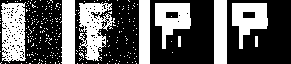
\includegraphics[scale=0.60]{./images/espureo.png}
\label{modelado}
\end{center}
\end{figure}

\begin{center}
\par Figura 1: Ejemplo de estado espúreo.
\end{center}

 Claramente se observa que la red converge a un estado espúreo.

\subsection{Patrones con ruido o incompletos}

\par El siguiente ejemplo muestra la respuesta de la red ante un patrón incompleto. Se utilizó una red asincrónica y se la hizo memorizar los archivos ``foot'', ``line1'', ``line2'', ``line3'', ``line4''\\.\\
A continuación se muestra el resultado de pasarle como entrada la imagen ``foot'' pero incompleta. En este caso particular se optó por borrar la mitad izquierda de la imagen: \\

\begin{figure}[H]
\begin{center}
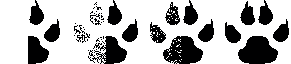
\includegraphics[scale=0.60]{./images/half.png}
\label{modelado}
\end{center}
\end{figure}

\begin{center}
\par Figura 1: Respuesta de una red de hopfield asincrónica ante un patrón incompleto.
\end{center}

\par Si en cambio se utiliza solamente ruido, en una red asincrónica que memorizó los patrones ``f'', ``h'', ``a'', ``footprint'' y le pedimos que evolucione partiendo de ``f'', la red rápidamente converge a la imagen deseada:

\begin{figure}[H]
\begin{center}
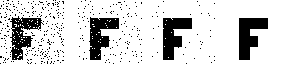
\includegraphics[scale=0.60]{./images/noisyf.png}
\label{modelado}
\end{center}
\end{figure}

\begin{center}
\par Figura 1: Respuesta de una red de hopfield asincrónica ante un patrón con ruido.
\end{center}



\subsection{Patrones invertidos}

\par En el siguiente ejemplo se muestran estados intermedios de la evolución de una Red de Hopfield asincrónica a la cual se la iniciaclizió con las siguientes imágenes provistas por la cátedra: ``line1'', ``line2'', ``line3'', ``line4'', ``h''.\\
La red neuronal en cuestión utiliza la mejora del bit de paridad como así también la inicialización a través de la matriz pseudo-inversa.\\
\par Utilizando la red neuronal antes descrita, se le pasó como entrada la imagen ``h'' invertida y con ruido. A continuación vemos su evolución; la primer imágen es el estado inicial, luego se ven dos estados intermedios y por último el final:\\

\begin{figure}[H]
\begin{center}
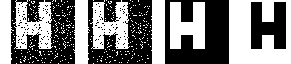
\includegraphics[scale=0.60]{./images/hinvypar.png}
\label{modelado}
\end{center}
\end{figure}

\begin{center}
\par Figura 1: Visualización de estados intermedios para una red de hopfield asincrónica con la mejora del bit de paridad y la utilización de la matriz pseudo-inversa
\end{center}

\subsection{Patrones desconocidos}

\par El siguiente ejemplo muestra la respuesta de la red ante un patrón desconocido. Se utilizó una red asincrónica y se la hizo memorizar los archivos ``line1'', ``line2'', ``line3'', ``line4''\\.\\
A continuación se muestra el resultado de pasarle como entrada la imagen ``h''  la cual la red no conocía: \\

\begin{figure}[H]
\begin{center}
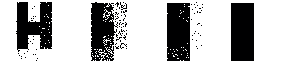
\includegraphics[scale=0.60]{./images/hnoinvnopar.png}
\label{modelado}
\end{center}
\end{figure}

\begin{center}
\par Figura 2: Respuesta de una red de hopfield asincrónica ante un patrón desconocido.
\end{center}


\subsection{Cantidad de patrones almacenables}
\par En una primer instancia, se intentó que la cantidad de patrones almacenables en la red 
sea similar a la capacidad sugerida teóricamente por Hertz en su libro, que corresponde a aproximadamente $0.138N$. Esto correspondería a más de 500 imágenes. Sin embargo esto no fue observado empíricamente.\\

\par La razón detrás de esta discrepancia entre lo teórico y lo práctico surge de asumir varias hipótesis al deducir dicho valor para la capacidad. En un primer plano, el valor surge de asumir que todos los patrones son azarosos. Como ya se ha explicado en la sección de matrices psuedo-inversas, este no es el caso para las imágenes tratadas; el término de crosstalk es mucho mayor en este caso que en el caso de tener patrones azarosos. En segundo lugar, el cálculo se refiere únicamente a la estabilidad en los estados atractores; surge de exigir que el error en los mismos sea menor a un $1\%$. Sin embargo no hace referencia a la posibilidad de que los patrones de entrada converjan a un estado espúreo, lo cual se observó seguido en la práctica al usar más de 6 o 7 imágenes.\\

\par El número exacto de cantidad de patrones máximos almacenables es difícil de determinar, dado que depende de qué patrones se usen. Patrones con mayor correlación (mayor término de crosstalk) por lo general traían mayores problemas. Además, se observó que la implementación psuedo-inversa tuvo resultados consistentemente mejores que la regla de Hebb.

\subsection{Comparacion Pseudoinversa vs Hebb}

Como ya se explicó anteriormente, la pseudoinversa por lo general obtuvo mejores resultados. Por ejemplo, en la siguiente figura 
se puede apreciar que la psuedoinversa obtuvo un buen resultado mientras que la red normal tuvo un 2% de error.

\begin{figure}[H]
\begin{center}
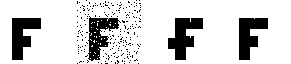
\includegraphics[scale=0.60]{./images/copara.png}
\label{modelado}
\end{center}
\end{figure}


\section{Conclusión}

\begin{itemize}
\item La cantidad de memoria requerida por al red de Hopfield es mucho mayor al tamaño de 
los patrones a almacenar.
\item La capacidad práctica de la red es mucho menor a la capacidad teórica, principalmente 
debido a la correlación entre patrones.
\item Se hallaron métodos para evitar que se converja a un patrón inverso.
\item El uso de la psuedoinversa obtuvo mejores resultados que la red de Hebb normal.
\end{itemize}




%----------------------------------------------------------------------


\clearpage
\onecolumn

\section*{Anexo A: Patrones}

\begin{figure}[H]
\begin{center}
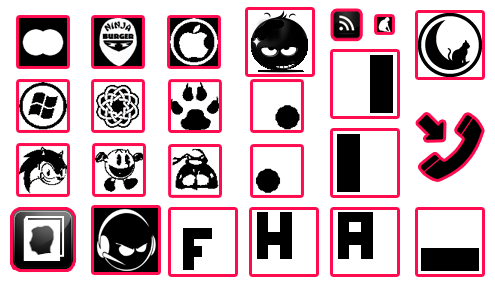
\includegraphics[scale=0.70]{./images/patterns.png}
\label{modelado}
\end{center}
\end{figure}

\begin{center}
\par Figura 1: Visualización de los 25 patrones con la que se inicializa a la red
\end{center}



%\VerbatimInput{./code/calculoAb.m}




\end{document}